\documentclass[11pt]{article}
\usepackage{hyperref}
\usepackage{graphicx}
\usepackage{float}
\usepackage[margin=0.5in]{geometry}

\hypersetup{linkcolor=blue,colorlinks=true}

\begin{document}
\begin{center}
\LARGE{\textbf{Specifications Document}}\\
\normalsize{Team 2 - CS374 - Fall 2014}
\end{center}
\vspace{.1in}

In this document, we describe the specifications for our Schedule Conflict Calculator application.
\vspace{.2in}

\LARGE Table of Contents \\

\normalsize
\begin{tabular}{| l || r |}
  \hline
  \nameref{sec:reqs} & Describes requirements of our product \\ \hline
  \nameref{sec:scenes} & Describes user interaction with our product \\ \hline
  \nameref{sec:dataflow} & Describes the interaction of modules within our product \\ \hline
  \nameref{sec:glossary} & Glossary of terms \\
  \hline
\end{tabular}

\pagebreak[4]

\section{Requirements} \label{sec:reqs}

Our Schedule Conflict Calculator Web application will function as an extension to other academic administration technologies. Given
a set of inputs related to moving a course from one time block to another, the application determines the number of student
scheduling conflicts that would arise in some number of move scenarios. The application handles a number of different move
scenarios, allowing the user to decide which scenario to test.

\pagebreak[4]

\section{Use Cases and Scenarios} \label{sec:scenes}

The user is allowed multiple scenarios for calculating schedule conflicts. For example, sometimes the user has a single
\textit{section-change description} in mind and would like to see scheduling conflicts. In other instances, a user might
know that they need to move a section to another time and/or room, yet would like to know which room out of a set of possible
candidates has the least number of conflicts.
\vspace{.2in}

\begin{figure}[h]
  \centering
  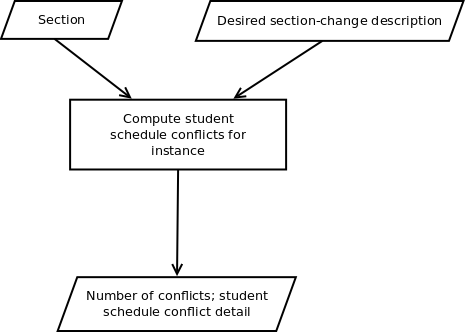
\includegraphics[width=0.5\textwidth]{diagrams/scenarioA.png}
  \caption{Describes a simple scenario for finding conflicts given a single section-change description}
\end{figure}

In the simple case, we consider a single section-change description supplied with a desired input section. Output will consist of the
number of conflicts as well as a detailed look at individual conflicts. If another section is already \textit{associated} with the
section-change description, the user is informed of the conflict but is still provided the normal conflict output as if there weren't
a course currently associated with the description. Other input parameters might be needed to provide a more customized operation tailored
to meet user needs.

\begin{figure}[h]
  \centering
  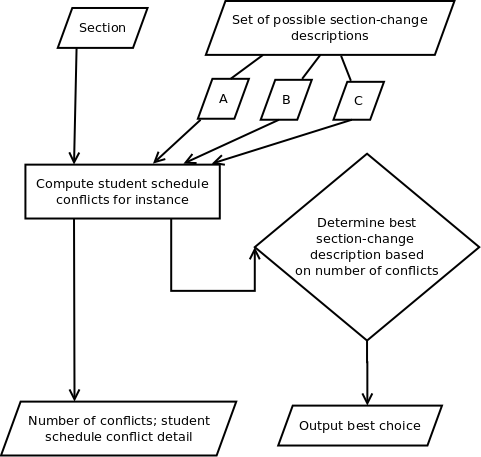
\includegraphics[width=0.5\textwidth]{diagrams/scenarioB.png}
  \caption{Describes a more complex scenario for finding conflicts given multiple section-change descriptions}
\end{figure}

Other scenarios are needed for more complex operations. A user might wish to provide a set of section-change descriptions to apply to
the input section in order to find the best change description. This set of descriptions may encompass multiple rooms and buildings and also
take into consideration moving courses already associated with section-change descriptions. This introduces added complexity. \\

To deal with this complexity, we introduce the terms \textit{locked-section} and \textit{floating-section} (see glossary). In the proposed
scenario (Figure 2), a set of section-change descriptions is provided into which the input section may be moved. In a simple case, the scenario
given in Figure 1 can be applied to each description. The description(s) with the fewest conflicts are then presented as output. However, sometimes
more than one section can be moved within the sections already associated with each section-change description. Each one of these sections is either marked
as a \textit{locked-section} or a \textit{floating-section}. A locked-section is one that cannot be moved. This automatically disqualifies the description to
which the locked-section is associated (conflicts are still computed as in the Figure 1 scenario). A floating-section may be moved within the set of 
section-change descriptions.

\pagebreak[4]

\section{Data Flow} \label{sec:dataflow}

This section describes the interaction of various modules within our application. We map the flow of data through the different
modules of the application, demonstrating how it is used and transformed.

\begin{figure}[h]
  \centering
  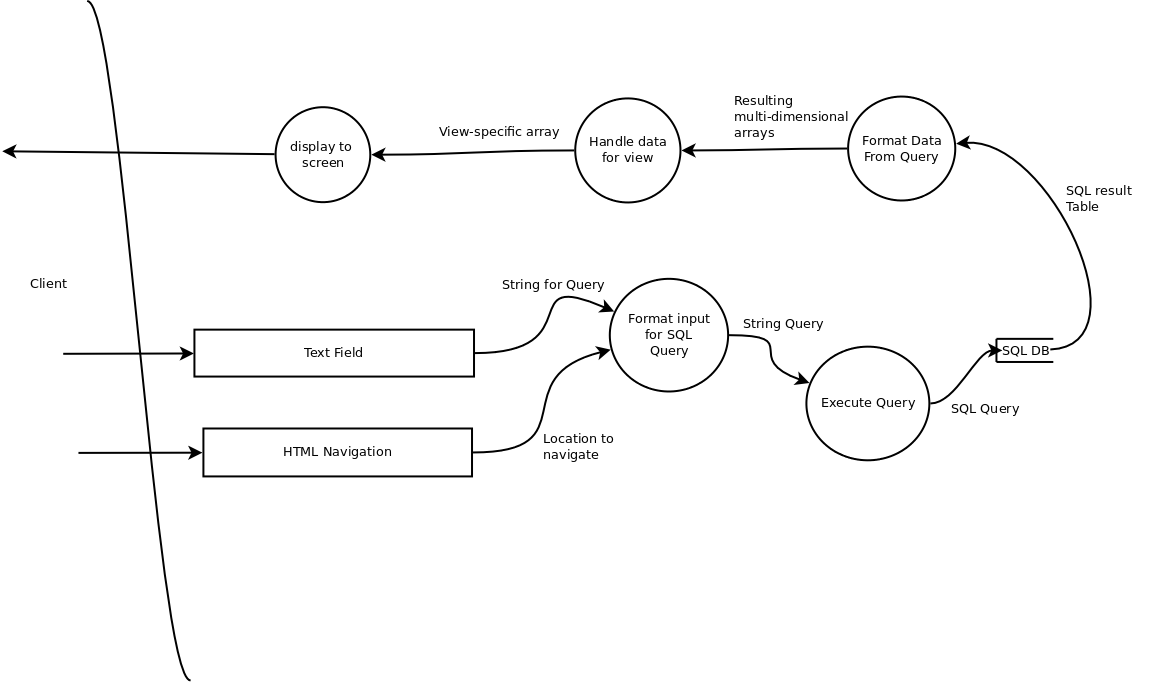
\includegraphics[width=1\textwidth,scale=1.5]{diagrams/dataflow.png}
  \caption{Data flow diagram for main application operation}
\end{figure}

\begin{figure}[h]
  \centering
  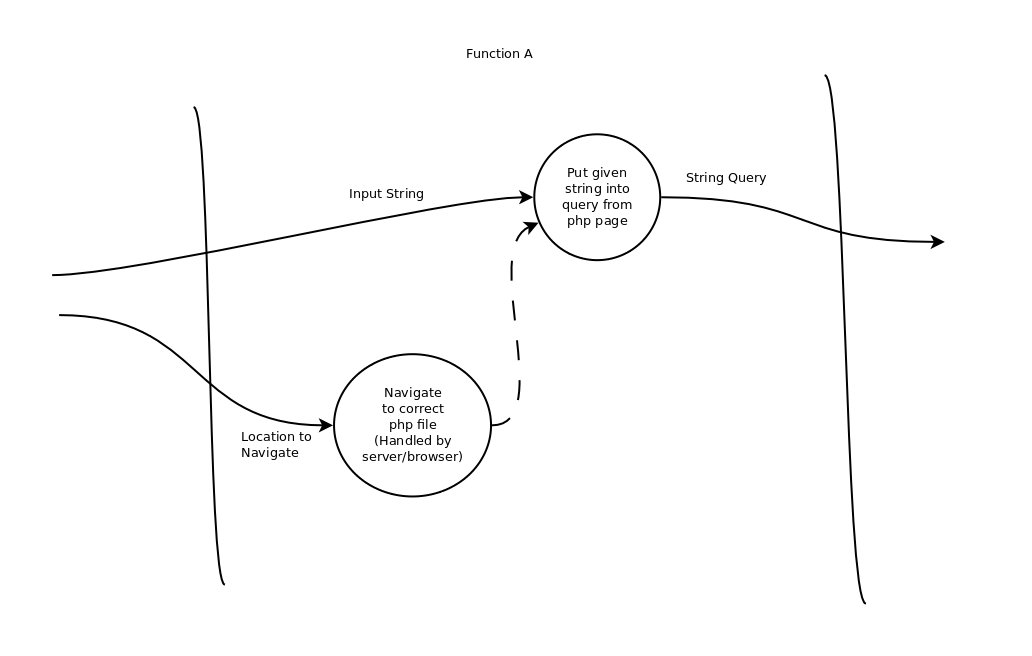
\includegraphics[width=.75\textwidth]{diagrams/FunctionA.png}
  \caption{Details function A in Figure 3}
\end{figure}

\begin{figure}[h]
  \centering
  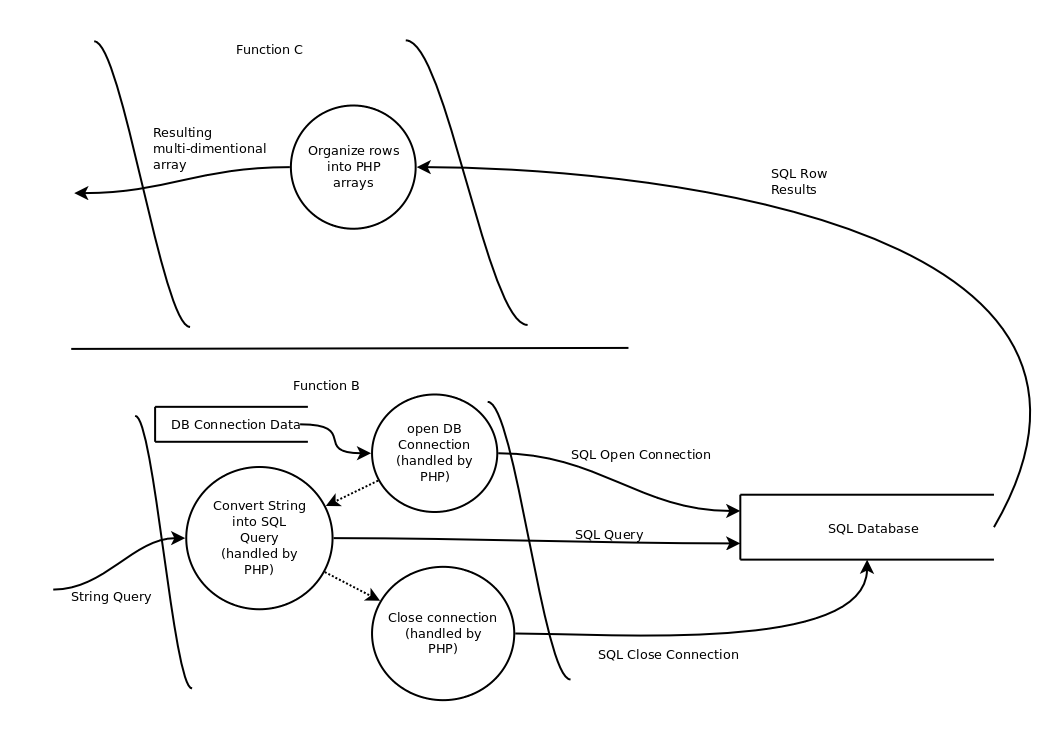
\includegraphics[width=.75\textwidth]{diagrams/FunctionsB&C.png}
  \caption{Details function B and C in Figure 3}
\end{figure}

\begin{figure}[h]
  \centering
  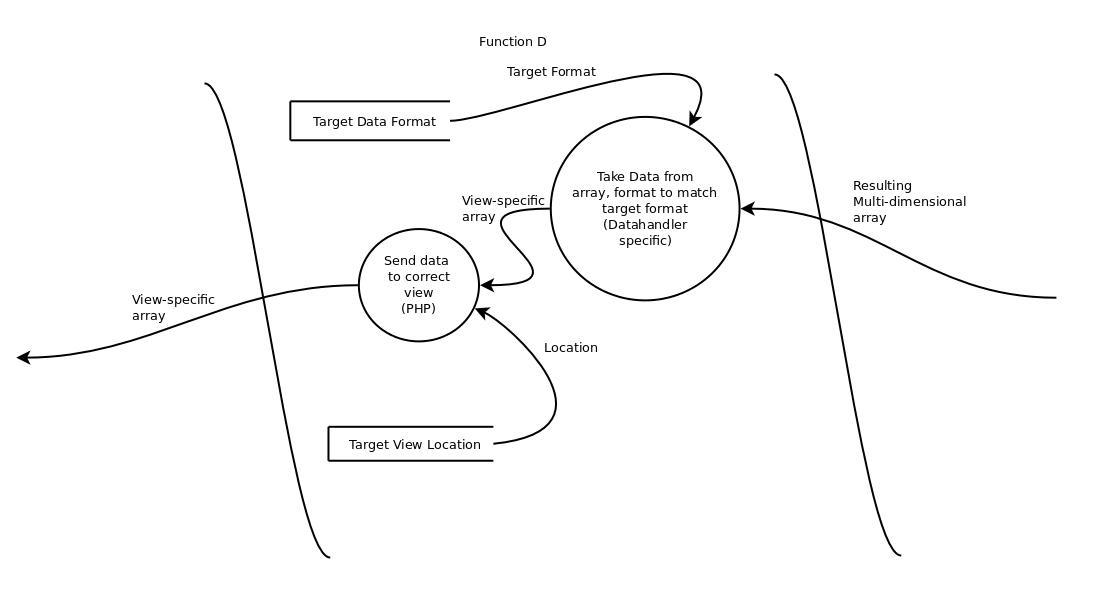
\includegraphics[width=.75\textwidth]{diagrams/FunctionD.png}
  \caption{Details function D in Figure 3}
\end{figure}

In each proposed scenario, a user provides input through an HTML form which is passed to a data handler. The data handler uses an
SQL database connection to issue a query and retrieve the data needed to execute the task. The handler is responsible for producing
the desired result. Different handlers will require different amounts and/or types of data and thus will make different queries. Handlers
will be implemented using a class hierarchy in PHP. Each derived class will implement a different handler-kind which executes a
distinct scenario. \\

\begin{figure}[h]
  \centering
  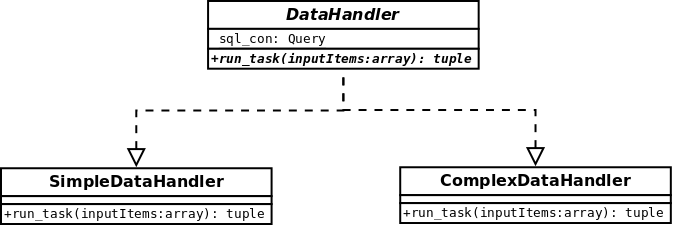
\includegraphics[width=.75\textwidth]{diagrams/data-handler-uml.png}
  \caption{Simple UML concept for data-handler class-hierarchy}
\end{figure}

Though each handler performs a different operation, it still functions according to the same interface. Figure 3 graphically
models data as it flows from the client, is transformed and goes back to the client as output. Figures 4-6 provide in more detail
the functions presented in Figure 3.

\clearpage
\pagebreak[4]

\section{Glossary} \label{sec:glossary}

\begin{description}
  \item[association] The set of courses whose location matches and time duration overlaps a section-change description
  \item[building] A collection of rooms.  Each building has a set of floors.
  \item[course] A general description of a class of sections.  Each course has a string (for the course type, such as CS or IT), and a number (such as 101), which can be either a string or an integer.
  \item[data-handler] An object that executes a scenario using data obtained from the database.  
  \item[floating-section] A section that may be potentially moved from either its current time, location or both.   This does not mean it can be moved from one instructor to another, nor can the section number change.
  \item[freshman] A student of Year 1.  It is preferable to move or change freshman classes rather than upperclassman classes, because there is more flexibility.
  \item[junior] A student of Year 3.  Less flexible than Freshmen and Sophomores, which means they should be changed after Freshmen and Sophomores, but unlike Seniors, it is not critical that they not be moved.
  \item[locked-section] A section that cannot be moved from its current time and location
  \item[professor] An instructor of a course; there is one professor per section
  \item[office-hours] A time block associated with a professor; a potential conflict item to consider.  If an instantiation of a course falls within time allotted to office hours, there is a conflict; this conflict is of less importance than conflicting course instantiations.
  \item[room] The meeting place of a section. Rooms are assigned to a Building.  Rooms cannot be reassigned, since they do not physically move.
  \item[scenario] A section change operation (e.g. moving a section from one time to another)
  \item[section] An instantiation of a course.  The number of sections starts at 01 and increases based on the number of classes that are to be taught for a given course such as CS101: CS101 01, CS101 02, etc.
  \item[section-change description] A tuple that specifies a desired change to a section's time and location.  Non-room changes have a hierarchy; change in a section's day implies change in time.  A change in professor implies change in day and change in time.
  \item[senior]A student of Year 4; due to the priority on graduation, seniors should not be moved unless as an absolute last resort.  Seniors who are in the second sememster of their year absolutely cannot be moved.
  \item[sophomore]A student of Year 2; not as flexible as Freshmen, but more movable than Juniors and Seniors.
  \item[student] A participant in a section.  Each student has a unique banner ID.  This banner ID is the key used.  Each student also has a Major, which determines appropriate courses that they can take.  Each student also has a Year: Freshman/1, Sophomore/2, Junior/3, and Senior/4.  Seniors cannot be moved, due to the importance of graduation.  Freshmen take the lowest priority; they should be moved before other classes.
\end{description}


\end{document}
